% Generated by paper/scripts/writing_sample_exhibits.py.
\begin{figure}[H]
\centering
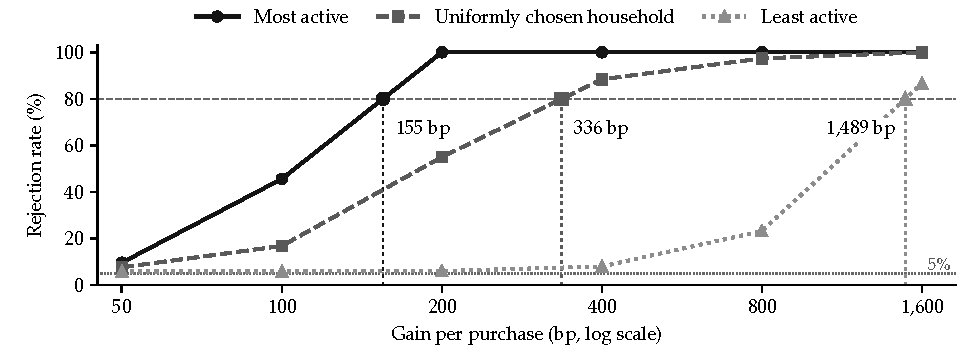
\includegraphics[width=\textwidth]{figures/writing_sample_power.pdf}
\caption{Power of the maximum-household test under the event-study benchmark at trade dates, 2015--2025. At each gain, the curves give rejection frequencies across 500 simulated trade-date datasets, with the gain added to every purchase of the most active household, a household drawn uniformly from the persistence sample, or the least active household. Labels mark the interpolated first 80\% crossing, with linear interpolation in log gain. Horizontal lines mark 80\% power and the nominal 5\% rejection rate.}
\label{fig:activity-detection}
\end{figure}
